\chapter{Marco Metodológico}

En este capítulo se pretende ahondar en la metodología utilizada para resolver el problema planteado desde el punto de vista de la gestión de proyectos, así como los cronogramas y métodos planteados para su solución.


\section{Desarrollo Orientado a Funcionalidades (FDD)}

La metodología elegida para la construcción de la plataforma planteada como problema en el Capítulo 1 fue el Desarrollo Orientado a Funcionalidades (FDD, por sus siglas en inglés) adaptado a una serie de entregas semanales, que sería reportadas los días sábado, desde el inicio del proceso de construcción de la plataforma, hasta el día de entrega, en la semana dieciséis (16) de desarrollo. Esta metodología fue elegida para facilitar el uso inmediato del sistema con sus funcionalidades actuales y, de esta manera, agilizar el proceso de pruebas de sistema, al realizarse en cada entrega.

El Desarrollo Orientado a Funcionalidades (Feature Driven Development o FDD) es uno de los llamados métodos ágiles dentro de la ingeniería del software, conocido por su alta adaptabilidad a los cambios y por sus tiempos de iteración cortos. Dicho método fue desarrollado por Jeff De Luca y Peter Code, y fue nombrado de esta manera en 1997 \cite{fdd}.
Goyal (2008) menciona que, en este enfoque, se asume que “cada etapa está 100\% completa antes de que la siguiente etapa comience” \cite{goyal2008}.
Por su parte, Khramtchenko (2004) destaca dos etapas principales de este proceso de desarrollo \cite{khramtchenko2004comparing}:
\begin{itemize}
    \item Descubrir la lista de funcionalidades a implementar.
    \item Implementación funcionalidad por funcionalidad.
\end{itemize}

Cada iteración dura alrededor de una a tres semanas, y al final de cada una de ellas se debe entregar una funcionalidad con la que el cliente pueda interactuar. Cada iteración, como se muestra también en la Figura \ref{figure:FDDworkflow} incluye el siguiente cuerpo formal:

\begin{itemize}
    \item Reunión inicial donde se especifican las funcionalidades requeridas.
    \item Proceso de diseño de clases, métodos y documentación.
    \item Revisión del diseño.
    \item Desarrollo de los métodos y las pruebas unitarias.
    \item Revisión del código.
    \item Despliegue de la funcionalidad.
\end{itemize}


\begin{figure}[H]
\centering
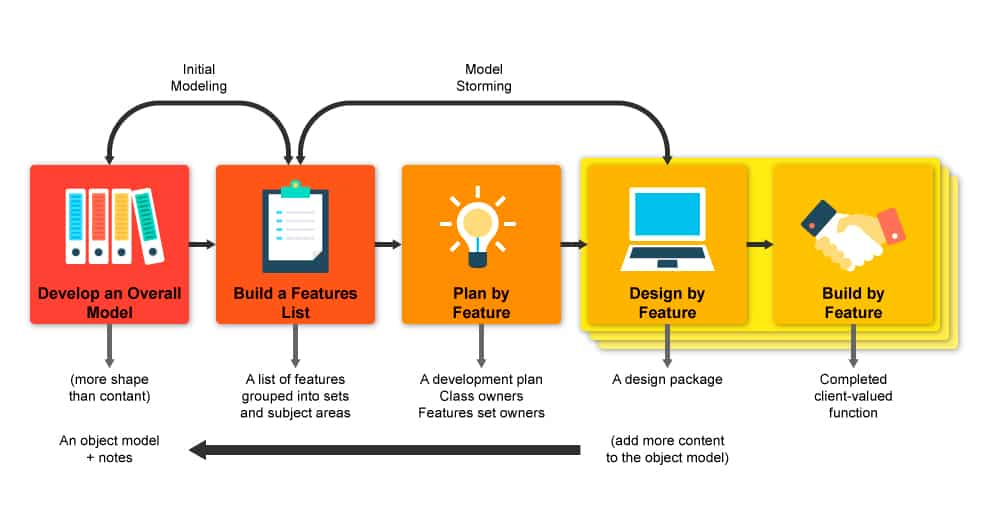
\includegraphics[width=0.80\textwidth]{img/5.png}
\caption{Plan de trabajo estándar del Desarrollo Orientado a Funcionalidades. Fuente: https://www.intellectsoft.net/blog/wp-content/uploads/Feature-Driven-Development-.jpg }
\label{figure:FDDworkflow}
\end{figure}


\section{Metodología FDD utilizada}

Para desglosar y sistematizar la metodología usada en el desarrollo de las funcionalidades de este producto, se procedió a hacer uso de un modelo propuesto por la Dynamic Domain Corporation \cite{fdd}. La misma divide la construcción del proyecto en cinco fases (entre paréntesis el porcentaje total de tiempo del proyecto invertido en cada fase), como se ve en la figura \ref{figure:FDDsteps}:

\begin{itemize}
    \item Desarrollar un modelo general. (14\%)
    \item Construir una lista de funcionalidades. (5\%)
    \item Planificar por funcionalidad. (4\%)
    \item Diseñar por funcionalidad.
    \item Desarrollar la funcionalidad. (77\%  tanto para diseño y desarrollo)

\end{itemize}

\begin{figure}[H]
\centering
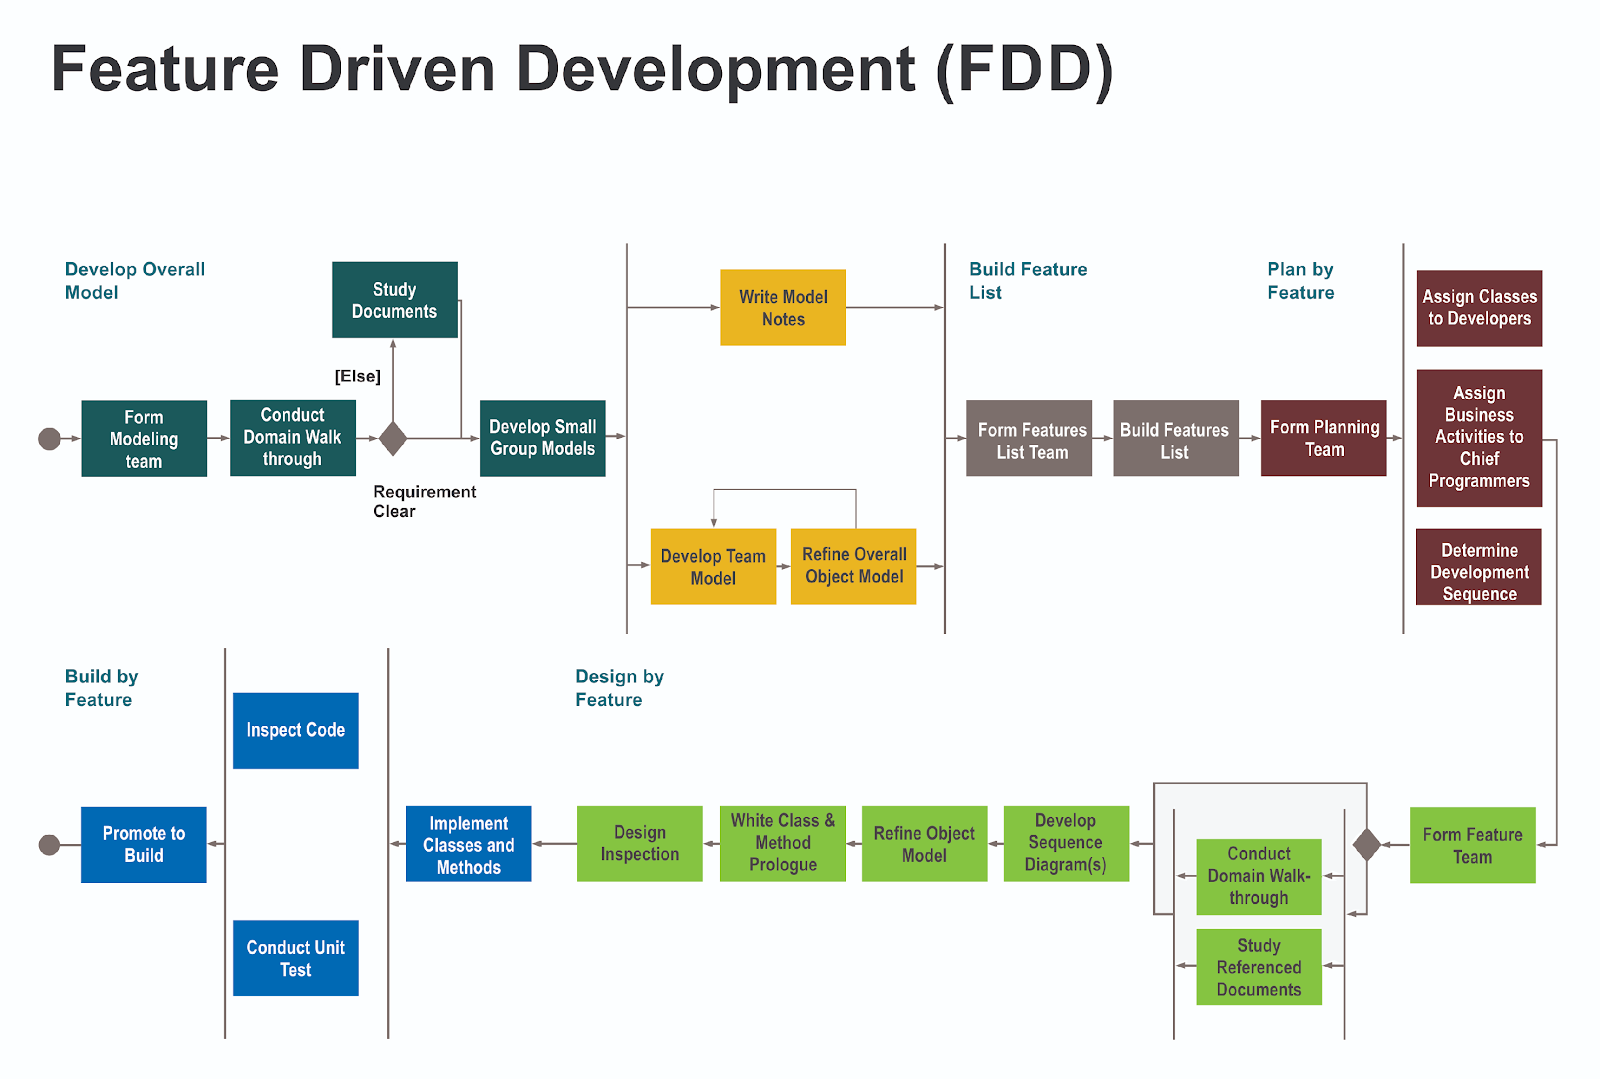
\includegraphics[width=0.80\textwidth]{img/6.png}
\caption{Pasos usados en la metodología FDD descrita por la Dynamic Domain Corporation (Fuente: http://thedynamicdomain.com/content/images/feature-driven.jpg)}
\label{figure:FDDsteps}
\end{figure}

En ese sentido, se postuló el siguiente cronograma de ejecución. Los requerimientos específicos serán detallados en el capítulo siguiente:

\subsection{Semana 1 a Semana 2: Modelo General}

\begin{itemize}
    \item Reunión inicial con el CEO de Ignis Gravitas para definir los objetivos iniciales del producto.
    \item Reuniones continuas para obtener los planos esquemáticos visuales de la arquitectura de la información (conocidos comúnmente como wireframes) así como para su validación.
    \item Reunión final para validación de los wireframes de la primera iteración.
    \item Obtención del modelo visual general de la aplicación.
\end{itemize}

\subsection{Semana 3: Lista de Funcionalidades y Especificaciones Generales}
\begin{itemize}
    \item Desarrollo de lista de requerimientos funcionales del producto a construir.
    \item Depuración de los diseños iniciales de las interfaces visuales.
    \item Generación del diagrama de despliegue.
    \item Generación del diagrama del diseño de datos.
\end{itemize}

\subsection{Semana 4 y 5: Autenticación}

\begin{itemize}
    \item Investigación sobre las herramientas disponibles y estándares de seguridad en autenticaciones.
    \item Diseño del diagrama de casos de uso para la autenticación.
    \item Implementación funcional de la API de autenticación.
    \item Implementación de las interfaces gráficas de usuario para el proceso de autenticación.
    \item Pruebas unitarias sobre la autenticación.
\end{itemize}

\subsection{Semana 6 y 7:  Publicaciones}

\begin{itemize}
    \item Diseño de diagramas de uso de las distintas publicaciones del sitio.
    \item Construcción de la vista principal de publicaciones.
    \item Definición y adaptación de la vista principal de búsquedas.
    \item Desarrollo de la interfaz gráfica para las publicaciones.
    \item Implementación de la API de publicaciones.
Pruebas unitarias y de integración sobre las publicaciones
\end{itemize}

\subsection{Semanas 8 y 9: Perfiles}

\begin{itemize}
    \item Construcción de diagramas de uso de los distintos perfiles del sitio.
    \item Construcción de las interfaces gráficas para los distintos perfiles especificados en las reuniones.
    \item Implementación de la API de perfiles.
    \item Pruebas unitarias y de integración sobre cada uno de los perfiles.
\end{itemize}

\subsection{Semana 10 y 11: Trabajos}

\begin{itemize}
    \item Construcción de diagramas de uso de la sección de búsquedas y muestra de trabajos.
    \item Construcción de las interfaces gráficas de la sección de trabajos.
    \item Implementación de la API de trabajos.
    \item Pruebas unitarias y de integración sobre la sección de trabajos.
\end{itemize}

\subsection{Semana 12 y 13: Productos}

\begin{itemize}
    \item Diseño de diagramas de uso de la sección de búsquedas y muestra de productos.
    \item Construcción de las interfaces de usuario de la galería de productos y propuestas de valor.
    \item Implementación de la API de productos.
    \item Pruebas unitarias y de integración sobre la vista de productos.
\end{itemize}

\subsection{Semanas 14 y 15: Pruebas de sistema}

\begin{itemize}
    \item Despliegue completo de la primera versión de la aplicación.
    \item Correcciones menores en reuniones constantes con los interesados del producto.
    \item Pruebas de sistema completas sobre toda la plataforma.
    \item Optimizaciones de pertinencia sobre la capa de interfaces y la capa de datos.
\end{itemize}

\subsection{Semana 16: Entrega del Producto}

\begin{itemize}
    \item Entrega final del producto.
    \item Planificación para mantenimiento del producto.
\end{itemize}